\documentclass[runningheads]{llncs}
\pagestyle{empty}
\usepackage{graphicx}

%Enricos packages
\usepackage{xcolor}
\usepackage{comment}
\usepackage{subfig}
\usepackage{graphicx}
\usepackage{amsmath,amssymb}
\usepackage{hyperref}
\usepackage{multirow}

\DeclareMathOperator{\Lagr}{\mathcal{L}}
\DeclareMathOperator{\RX}{\mathbb{R}}
\DeclareMathOperator{\BigO}{\mathcal{O}}

\newcommand{\xmark}{\text{\ding{55}}}



\begin{document}

\title{$DATE$: Derivative Alignment Training for Extrapolation with Neural Networks}

\author{Enrico Lopedoto 
\and Tillman Weyde\and Kizito Salako}
\authorrunning{E. Lopedoto, T. Weyde, K. O. Salako}

\institute{City, University of London \\
Department of Computer Science\\
Northampton Square, London, UK \\
\email{\{enrico.lopedoto,t.e.weyde,k.o.salako\}@city.ac.uk}}

%%%%%%%%%%%%%%%% CHECK EMAILS

\maketitle 
\begin{abstract}

In this work we introduce $DATE$ (Derivative Alignment Training for Extrapolation), a method to improve the extrapolation behaviour of neural networks (NN) with Rectified Linear Unit activation (ReLU) on univariate regression tasks. 
ReLU NNs naturally lend themselves to linear extrapolation beyond the training data range. 
However, there are two known limitations of extrapolation properties of trained ReLU NNs, that we address in this paper. 
When minimising the error of the prediction, the derivative of the NN model function can still show high variation, which can cause variable extrapolation. 
Non-linearities of the model function outside the training data range can lead to inconsistent extrapolation behaviour.
In prior work, the extrapolation issue has been addressed with a set of regularisation functions, called $ReLEx$. 
To improve extrapolation and interpolation, we introduce two new regularisation terms: $D1$-loss and $IR$-loss. 
The $D1$-loss directly penalises the deviation of the model derivative from a target derivative as estimated from the data by interpolating between neighbouring data points. 
The $IR$-loss penalises positions of the non-linearities of the ReLU units outside a given range. Optimising the combination of $D1$ with $IR$ loss and/or some of the $ReLEx$ functions constitutes the $DATE$ method.
We evaluate $DATE$ on regression tasks with noiseless data generated from analytic functions. 
We test different $DATE$ configurations and find that training with $DATE$ can reduce the variability of the model slope, prevent non-linearities outside the training data range, and improve extrapolation consistency as measured by different metrics. 
The most effective $DATE$ variants also have reduced complexity compared to $ReLEx$.

\keywords{Extrapolation \and Regression \and Neural Networks \and Derivative.}

\end{abstract}

%%%%%%%%%%%%%%%%%%%

\section{Introduction}

\begin{figure}[t]
 \centering 
 \subfloat[5 trained NNs]
 {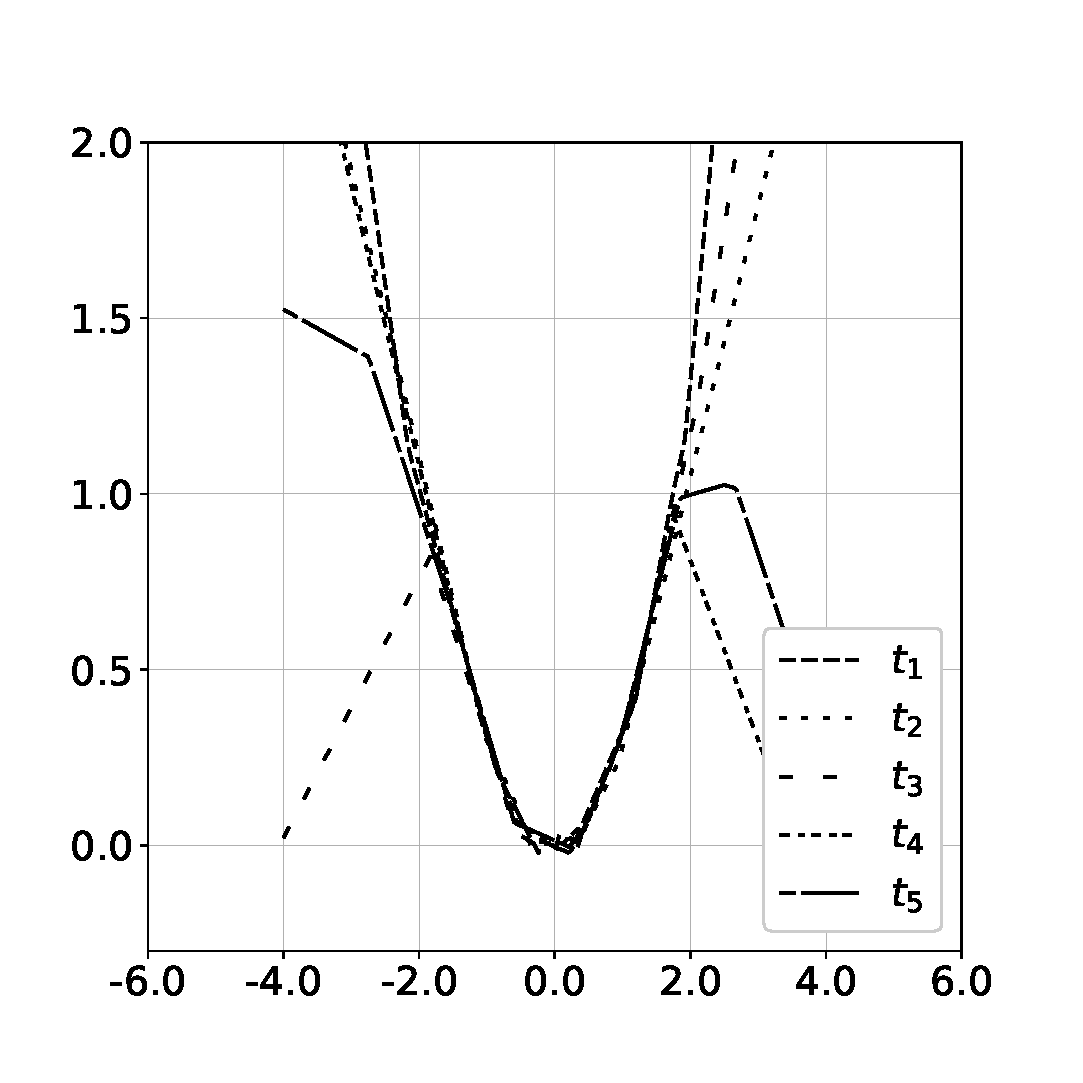
\includegraphics[trim={1cm 1cm 1cm 1.9cm},clip, width=0.51\linewidth]{pics/SpagPred_pow_MSE__96355ae8-7134-11ef-8273-4b5d8eb7968f.eps}}
 \subfloat[Value and slope of a single NN]
 {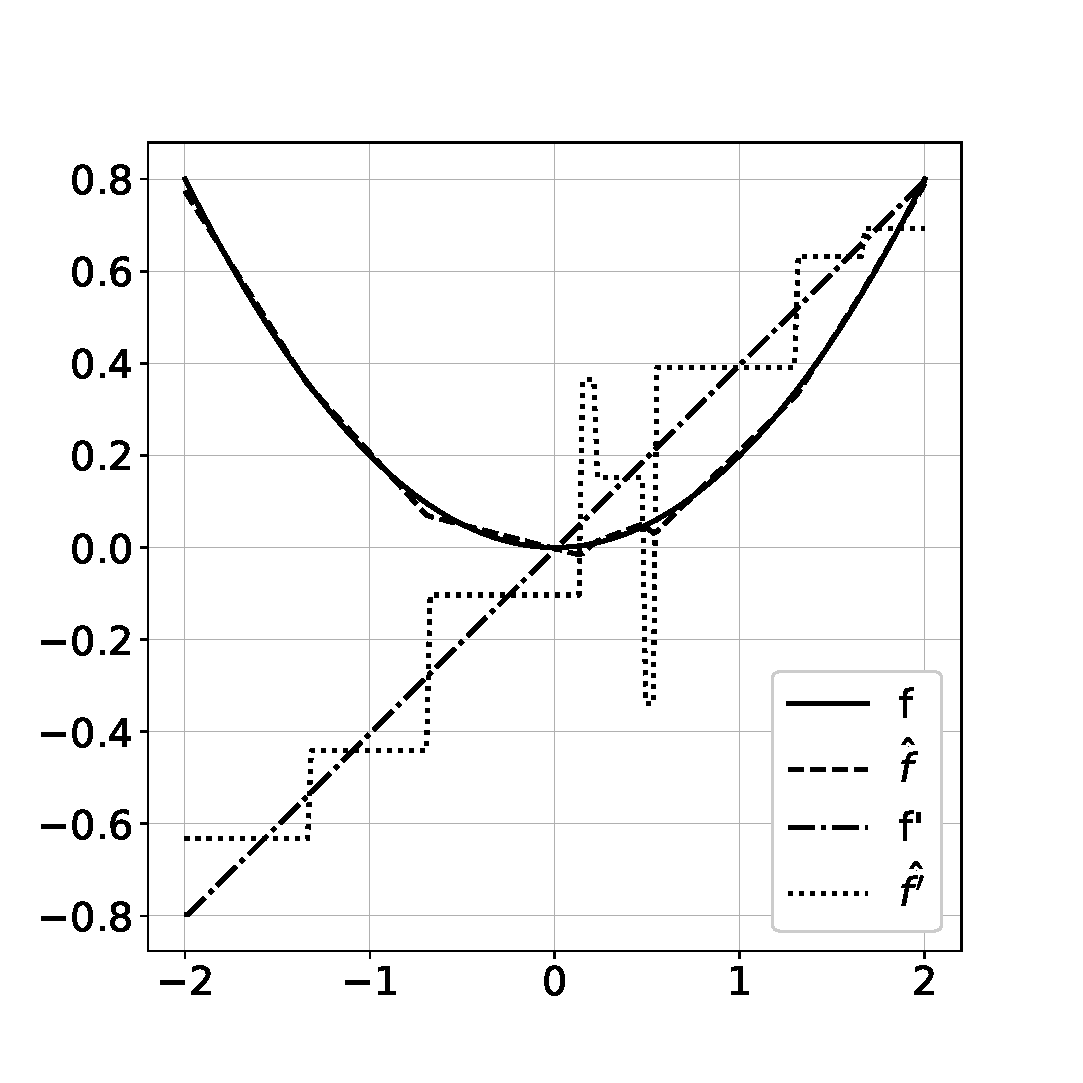
\includegraphics[trim={0.5cm 1cm 1cm 1.9cm},clip, width=0.51\linewidth]{pics/DerivPlot_pow_MSE__96355ae9-7134-11ef-8273-4b5d8eb7968f.eps}}
 \caption{(a) Extrapolation in the range [-4,4] of a quadratic function with data trained in the range [-2,2] with a ReLU NN trained with MSE loss only. 
 (b) we display the interpolation range [-2,2] true function (solid), the model function (dashed), the slope of the target function (dashdotted) and the slope of the model function (dotted).
 }
 \label{fig:runs_non_good}
\end{figure}

In supervised machine learning the immediate objective is to fit the model function to the training data by minimising a loss function. 
This loss function is typically defined in terms of the values of the data and the model, and for regression the error metric is typically the mean squared error (MSE). 
The most popular machine learning models in recent years have been neural networks (NN). 
In particular, NNs with rectified linear unit (ReLU) activation have desirable properties in terms of computational efficiency and conceptual simplicity so that ReLU has become the standard activation function \cite{goodfellow2016deep}.

Here, we are concerned with the extrapolation of the model beyond the range of the training data. 
We explore specifically linear extrapolation behaviour, which is made possible by the ReLU activation function as opposed to previously more common sigmoid functions (logistic function and tanh). 
When training ReLU NNs to minimise the MSE, there are two problems that can be observed in \autoref{fig:runs_non_good}:
(a) shows predictions inside and outside of the training data range [-2,2] of five separately trained NNs with one hidden layer of $10$ neurons, and we observe a wide variation of behaviour outside the training data range, at least for some models; 
(b) shows the value and slope of the model vs the target function in the training data range, where the slope of the model function deviates in some places far from the true slope value. 
A solution to the extrapolation problem (a) has been proposed in the $ReLEx$ method \cite{Lopedoto20}, which, however, increases the computational complexity of the training and exacerbates the derivative deviations (b).

The goal of this work is extend and improve over $ReLEx$ with a method that achieves desirable linear extrapolation as well as interpolation behaviour in standard ReLU neural networks more effectively, more efficiently and with fewer changes compared to standard neural network learning. 

Our contributions are as follows: 1)~we introduce improved extrapolation of NN models through derivative alignment; 
2)~we propose $DATE$, a new method to improve extrapolation in regression task with ReLU neural networks including two new regularisation terms, $\Lagr_{D1}$ and $\Lagr_{IR}$; and 
3)~we provide an implementation of $DATE$ in PyTorch and an evaluation of learning five different target functions with simple NNs using $DATE$.

\section{Related Work}

In supervised machine learning, over the last decade, neural networks (NN) have been adopted for many machine learning problems~\cite{goodfellow2016deep,Fan2019ASO}. 
However, neural networks display differences in behaviour when predicting a function between data points and predicting a function for points outside the range of the training data. 
We refer to prediction in the training data range as \emph{interpolation} and outside the training data range as \emph{extrapolation}, (see, e.g., \cite{Abiodun2018}). 
Some methods to address the extrapolation problems for mathematical functions have been proposed by
\cite{Sahoo2018} and \cite{Madsen2020}, who introduce non-standard NN models with activation functions such as identity and multiplication functions and achieve improved extrapolation.

A lack of extrapolation has also been observed in the context of linguistic structures, where rules are not generalised between different words or syllables \cite{LakeBaroni2017,Suzgun2019,Li2018,mitchell2018extrapolation}, or when we need to extrapolate from even to odd numbers \cite{Marcus1999}, or when extrapolating Dyck language recognition to long sequences \cite{ElNaggar2023TheoreticalCA}.

%%%%%%%%%%%%%%%%%%%%%%%%%%%%%%%%%%%%%%%%%%%%%%

\subsection{Extrapolation with ReLU NNs}

The rectified linear unit ($ReLU$) function is the most popular activation function in modern neural networks \cite{goodfellow2016deep}, firstly introduced by \cite{fukushima1975relu} to the best of our knowledge. 
The ReLU activation offers the possibility of performing unbounded linear extrapolation that is not possible with bounded activation function like the logistic sigmoid or $tanh$ functions. 
However, NNs trained with MSE using ReLU show high variability in the extrapolation, as illustrated above.

There is no single ideal extrapolation behaviour in the absence of a known function outside the training data range. 
As we have decided to limit ourselves to linear extrapolation, a possible target is the tangent line at the data point or points. 
In addition, there are considerations with respect to the learning process of NNs, where we adopt the desiderata from \cite{Lopedoto20}: 
\begin{itemize}
 \item the NN should learn how to extrapolate from the training data;
 \item the NN should adapt the learning process making as little changes to the network structure, activation functions and training process as possible;
 \item the method and implementation should be easy for practitioners to replicate and use.
\end{itemize}
We also adopt the design decision of \cite{Lopedoto20} to address the problem by changing only the loss functions and not the structure of the NN itself. 

\subsection{Simple ReLU NNs and \emph{dying ReLUs}}

From here on, we consider a simple feed-forward ReLU neural network with a single input, a single hidden layer (comprising $H$ neurons), and a single output that calculates the function
$f(x,\boldsymbol{\beta}) =
b_{o} +\sum^{H}_{h=1} w_{ho} \cdot ReLU(w_{h} x + b_{h}) $, where $w_{h}$ and ${b}_{h}$ are the weight and bias value of hidden neuron $h$, respectively. 
The weight between hidden neuron $h$ and the output neuron is $w_{ho}$, while $b_{o}$ is the bias of the output neuron. All these weights and biases make up the vector $\boldsymbol{\beta}$. 
We will also write $\hat{y}$ in short for $f(x,\boldsymbol{\beta})$.

The ReLU function, $ReLU:\mathbb{R}\rightarrow\mathbb{R} = max(x,0)$, has two parts, for negative arguments the output is constant $0$, we call this the \emph{constant part} of the ReLU.
For positive inputs $x$, the output is $x$ and we call this the \emph{linear part} of the ReLU. 
At input $0$, the ReLU is not differentiable, this is often referred to as the \emph{non-linearity} of the ReLU or the \emph{0-point} as defined below. 

A known problem in NN learning is a \emph{dying ReLU}, as described in \cite{douglas2018relu,lu2019dying}. 
This refers to a situation where all training data points lead to a negative input to the ReLU function, so that it operates only in its constant part, where its output is $0$ and its derivative is $0$.
In this situation, the input weights of that neuron will not be changed during learning by gradient descent.
The linear part of that neuron will therefore not depend on the data but only on the initialisation of the weights. 
Examples of this are the observed variation of slopes outside the data range in \autoref{fig:runs_non_good}(a), where we plot the output over the range [-8,8] of the 5 NN training runs with different random initialisation. 
The specifics of the data, networks and training are described below in \autoref{sec-experiments}.
In (b), we plot the output value and slope of a single trained NN and of the target function.

\subsection{$ReLEx$ and \emph{0-points}}

$ReLEx$, introduced in \cite{Lopedoto20}, is a method that aims to control extrapolation behaviour by introducing additional loss functions, which mainly control the position and orientation of the ReLU function in the hidden neurons.
The results show that the usage of the proposed loss functions improves the extrapolation behaviour, but the method has limitations and requires tuning of several parameters. 
In addition, these loss terms increase the computational complexity compared to training with MSE alone. 

The \emph{ReLEx} method, is focused on \emph{0-points}, i.e., the points in the input space where the ReLU's constant and linear parts meet and where the ReLU function is non-linear. 
Formally, the \emph{0-points} are the input values $x_{h0}$ that lead to input $0$ for a hidden neuron~$h$: $0 = w_{h} \cdot x_{h0} + b_{h}$, so that the \emph{0-point} for hidden neuron~$h$ is $x_{h0} = -b_{h}/w_{h}$. 

The \emph{ReLEx} regularisation introduces four individual loss terms $\Lagr_l$ with associated scaling parameters $\theta_l$. 
They serve different purposes which we describe here briefly. 
The formal definitions are listed in \autoref{tab:my_relexlosses}.
The \textbf{Centripetal} loss ($\Lagr_{CP}$) pulls all the \emph{0-points} inside the training data range; the 
\textbf{Mutually Repellent} loss ($\Lagr_{MR}$) is responsible for counter balancing the $\Lagr_{CP}$ force by distributing the \emph{0-points} inside the training data range; 
the \textbf{Weight Orientation} loss ($\Lagr_{WO}$) moves the \emph{0-point} for each ReLU so that the constant part covers most of the data points and only data points close to the margins of the training data range determine the slope of the extrapolation; 
lastly, the \textbf{Weight Sign} loss ($\Lagr_{WS}$) recovers from the degenerate case when all the weights have the same sign (occurring on average only in $1$ out of $2^{H-1}$ random initialisation of a network with $H$ hidden neurons).

\begin{table}[t!]
 \centering
 \begin{tabular}{lclcc} \hline
 Loss Name & Symbol & Definition & Complexity \\
 \hline \hline
 Centripetal & $\Lagr_{CP}$ & $\sum_{h=1}^H \sum_{k=1}^K (x_{h0} - x_{k})^2$ & $O(H K)$ \\
 \hfill
 \\
 Mutually Repellent & $\Lagr_{MR}$ & $\sum_{h=1}^H \sum_{j>i}^H \frac{1}{(x_{h0} - x_{j0})^2+ \varepsilon}$ & $O(H^2)$ \\ 
 \hfill
 \\
 Weight Orientation & $\Lagr_{WO} $ & $- \sum_{h=1}^H {ReLU((x_{h0} - \bar{x})\cdot w_h + \varepsilon)}$ & $O(H)$ \\
 \hfill
 \\
 Weight Sign & $\Lagr_{WS} $ & $({\sum_{h=1}^Hw_h})^2$ & $O(H)$ 
 \\
 \hline
\end{tabular}

\caption{The loss terms used in ReLEx improve extrapolation. 
$K$ is the number of data points.
$H$ is the number of hidden neurons. 
$x_{h0}$ is the \emph{0-point} of hidden neuron $h$ (dependent only on the network weights $w_h$ and $b_h$).
$\bar{x}$ is the average of the training data. 
The complexity refers to a single calculation of the loss value. 
}
\label{tab:my_relexlosses}
 
\end{table}


\section{$DATE$~--- Derivative Alignment Training for Extrapolation}

In this work, we explore a new approach to improve extrapolation, which involves directly controlling the slope of the model function, and also a new approach to avoid \emph{0-points} outside the data range.
This helps to solve the two issues of NNs for extrapolation illustrated previously (\autoref{fig:runs_non_good}). 
To avoid the 0-points outside the training data range, i.e. \emph{dying ReLUs}, as shown in 1(a), we introduce a new efficient loss term $\Lagr_{IR}$.
To improve the alignment of the slope of the target and model, as shown in 1(b), we introduce a new loss term $\Lagr_{D1}$. 
Optimising the combination of $D1$ and $IR$ losses constitute the $DATE$ method.

\subsection{$\Lagr_{D1}$ }

The concept of derivative alignment has been introduced in \cite{lopedoto2024derivativebased} with a special regularisation term, the $DLoss$.
Here, we introduce $D1$-loss -- $\Lagr_{D1}$ -- a univariate version of $DLoss$. 
Like $DLoss$, $\Lagr_{D1}$, penalises the deviation of the model's derivative from the target function derivative estimated from the training data points.
More formally, it is the sum of the squared differences between the model derivative $\hat{f}'$ -- the first derivative of the model function $\hat{f}$ -- and an estimate of the target derivative $y'$, based on the training data.

While $DLoss$ uses sampling in the multi-dimensional case, there is a total order of the input data in the univariate real case, so we can define the data vector $XY = [(x_1,y_1), \ldots , (x_K,y_K)]$ ordered by the values of $x$.

Then, we estimate the first derivative of the target function $y'$ at $k-1$ points $x'$ as the vector of pairs 
\begin{equation}
 XY' := [(x'_1,y'_1,), \ldots , (x'_{k-1},y_{k-1}')] 
\end{equation}
where 
\begin{equation}
 (x'_k,y_k') = \bigg((x_{k+1}+x_k)/2,(y_{k+1}-y_{k})/(x_{k+1}-x_{k})\bigg) ,
\end{equation}
i.e., we take $y'_k$, the slope of the line between two data consecutive points, as the derivative value for argument $x'_k$, the mid-point between two consecutive $x$-values.

Without additional assumptions, we do not know anything about the true target function except for the provided data and, thus, cannot give any guarantees on how far the estimated derivative $y'$ may be from the true derivative. 
However, if the true function $f$ is differentiable, we do know that $y_{k+1}'$ is the derivative value $f'(x)$ for some $x \in [x_k, x_{k + 1}]$ by the mean value theorem.

We calculate the model derivative $\hat{f}'$ using the finite difference method with a parameter $\varepsilon$ as 
\begin{equation}
 \hat{f}'(x) = \frac{ \hat{f}(x+\varepsilon)-\hat{f}(x-\varepsilon)}{2\varepsilon}.
\end{equation}
We use $\varepsilon = 0.05$ as it is large enough to avoid numerical issues and suitable for the curvature of the functions that we use in our experiments here. 
$\Lagr_{D1}$ is then defined as 
\begin{equation}
 \Lagr_{D1} = \sum_{(x',y') \in XY'} \big(y' - \hat{f'}(x')\big)^2
\end{equation}
and with it we are able to approximate the local slope of the model function to the local slope of the data with complexity of $O(H K)$.

\subsection{$\Lagr_{IR}$ }

In \autoref{fig:runs_non_good}(a) we saw undesired behaviour outside the data range.
We are interested in making sure that at least two data points are covered by the linear part of every ReLU, so that the slope of the model in the extrapolation range will be determined by the data. 

To do so, in $ReLEx$, $\Lagr_{CP}$ tries to pull the 0-points inside the training range.
For higher $\theta_{CP}$ values, however, we have observed that all 0-points cluster around the data mean. 
To counterbalance this effect $\Lagr_{MR}$ was introduced to equally distribute the 0-points over the range.

To avoid \emph{0-points} outside the training data range, we introduce the Internal Range loss $\Lagr_{IR}$ defined as:
\begin{equation}
 \Lagr_{IR} = \sum_{k=1}^K \big(ReLU(-x_{k0} + L - \tau) + ReLU(x_{k0} - R + \tau)\big)^2, 
\end{equation}
where $K$ is the number of hidden neurons, $L$ and $R$ are the most left point and right point of the training data range respectively and $\tau$ defines the margin from where data points within the training data range are covered.
This loss pulls the 0-points outside the training data range toward the inside with margin $\tau$. 

Only hidden neurons where the 0-points fall outside of the training data range with a margin $\tau$ are affected by $\Lagr_{IR}$ as opposed to $\Lagr_{CP}$, where stronger weight drives 0-points toward the mean of the data set and $\Lagr_{MR}$ distributes them, making the calibration of their relative weights necessary. 

Another benefit of using $\Lagr_{IR}$ is that it has computational complexity $O(K)$. 
It fulfils the same function as $\Lagr_{CP}$ combined with $\Lagr_{MR}$ complexity is $O(H^2)$. While the $O(H K)$ complexity of $\Lagr_{CP}$ could be reduced to $O(H)$ by using the mean of the data instead of the individual points), 
$\Lagr_{MR}$ has complexity $O(H^2)$ that cannot be reduced directly. 

%%%%%%%%%%%%%%%%%%%%%%%%%%%%%%%%%%%%%%%%%%%%%%%%%%%%%%%%%%%%%%%%%%%%%%%%%%%%%%%%%%%%%%%%%%%%%
\section{Experiments}\label{sec-experiments}

We evaluate the effect of three different $DATE$ configurations by training a small ReLU NN on data sampled from analytical functions. 
The baselines are standard NNs with $MSE = \frac{1}{n}\sum_{y \in Y} (y - \hat{y})^2$ 
 and $ReLEx$ losses (as described above).
We run different experiments with settings described below.

\textbf{Method.}
We chose ReLU-based NN with a single input, single output, and one hidden linear layer with $10$ neurons. To train it we use the Adam optimiser.

\textbf{Data generation.}
For this paper, we only consider noise-free data points sampled from a specific mathematical function $f(x)$. 
The training data range of the input $x$ is $[-2, 2]$ with a fixed grid of $200$ equidistant points. 
We use five different functions $lin$ $f(x) = x$, $abs$ $f(x) = |x|$), $pow$ $f(x) = \frac{1}{5}x^2$, $sigm$ $f(x) = 1 / (1 + e^{-x})$), and ($sin$ $f(x) = \sin(x)$). 

\textbf{Hyper-parameters.}
We use the following hyper-parameters for the training: learning rate $\epsilon = 0.007$; momentum $\nu = 0.9$; and $700$ epochs with mini-batch size $20$. These parameters have shown in preliminary experiments to reliably achieve convergence without major instabilities during the training process.
We varied $\theta_{D1}$ = $\{0.1,0.3,0.5,0.7,0.9\}$ to explore the effect of $DATE$.
For the other losses the parameters that we use in the experiments are those found in \cite{Lopedoto20} to work well, specifically $\theta_{CP} = 0.3$, $\theta_{MR} = 10$, $\theta_{WO} = 0.3$, $\theta_{WS} = 0.1$ and $\theta_{IR} = 5$. 


\subsection{Evaluation metrics}

We use two types of metrics: interpolation and extrapolation metrics.

\paragraph{Interpolation metrics} are calculated on the training data range [-2,2] where we use 200 equidistant samples:
\begin{itemize} 
 \item \textbf{$MSE_{int}$}: MSE of prediction against true value on a 200 feature points sampled from a uniform distribution in the training data range;
 \item \textbf{$MSE_{D1}$}: MSE of model derivative against $y'$ on a 200 feature points sampled from a uniform distribution in the training data range.
\end{itemize}

\paragraph{Extrapolation metrics} are calculated on the \textit{extrapolation set}, which consists of 200 points, 100 sampled from a uniform distribution in the left $[-10,-2]$ and 100 from the right $[2,10]$ extrapolation range.
We calculate these metrics individually for the right and left extrapolation set and their average. 

The ranges of values the margins that determine the interpolation can make a difference both for the extrapolation and the measurement. 
We can use a wider range from the margin or use more local information. 
Less local extrapolations will be more robust against noise in the data, but further away from the tangent at the last data point. 
Therefore we use a spectrum of targets to measure the precision of extrapolation.
This is reflected in the different metrics calculated on the extrapolation data range: 
\begin{itemize} 

 \item \textbf{$Tan_{ex}$}: MSE of prediction against the tangent lines to the target function at the margins of the training data range. 
 \item \textbf{$WLR_{ex}$}: MSE of the model prediction against a weighted linear regression (WLR) over the data points near the margin.
% The WLR is a regression where we assign a different weight to each input.
 In the WLR, we over-weight data closer to the margins of the training data range.
 The weighting scheme used is as per \cite{Lopedoto20} section 5.1, defined by a exponential function which allocates weights rising exponentially toward the margin $L$ and $R$ of the training data range.
 The weights are normalised to sum up to 1.
 \item \textbf{$D1_{ex}$}: MSE of the model prediction against the line of the last two point with slopes $y'_{1}$ for and $y'_{k-1}$.
 
\end{itemize}

The metrics reported are the average values obtained from $10$ runs for each experiment.
In addition, we measure extrapolation consistency with the standard deviation of the slope of the linear regression over the $(x,\hat{y})$ points in the extrapolation set. 
We do this, as before, separately on the negative and positive extrapolation ranges. 

\begin{itemize}
 
 \item \textbf{$\sigma_{S}$}: is the extrapolation variability over $10$ runs. It is calculated as the standard deviation of the slope resulting from the linear fitting over the predicted values in the portion $S$ of the extrapolation range, i.e. $[-10,-2]$ for left and $[2,10]$ for right.
\end{itemize}


%%%%%%%%%%%%%%%%%%%%%%%%%%%%%%%%%%%%%

\subsection{$DATE$ Configurations}

We compare different configurations of $DATE$ in order to evaluate the effects of $\Lagr_{D1}$ and $\Lagr_{IR}$.
We test MSE and $ReLEx$ and three other different variants of $DATE$. 
Below we describe each configuration.

\paragraph{$DATE_1$: Full $ReLEx$ + $\Lagr_{D1}$. }
Here, we add $\Lagr_{D1}$ to all $ReLEx$ loss terms. 
We hypothesise that $\Lagr_{D1}$ will improve the derivative alignment and, thus, lead to better extrapolation. 
The total loss function $\Lagr$ is defined as:
\begin{equation}
 \Lagr = ReLEx + \theta_{D1}\Lagr_{D1} + MSE
\end{equation} 

\paragraph{$DATE_2$: $\Lagr_{WO}$ + $\Lagr_{WS}$ + $\Lagr_{IR}$ + $\Lagr_{D1}$ }
In this loss configuration, we replace the $\Lagr_{CP}$ and $\Lagr_{MR}$ terms that are part of $ReLEx$ with $\Lagr_{IR}$. 
We hypothesise that this configuration should improve the adaptability within the training data range compared to the $ReLEx$ and $DATE_1$.
The total loss function $\Lagr$ is defined as:
\begin{equation}
 \Lagr = \theta_{WO}\Lagr_{WO} + \theta_{WS}\Lagr_{WS} + \theta_{IR}\Lagr_{IR} + \theta_{D1}\Lagr_{D1} + MSE
\end{equation} 

\paragraph{$DATE_3$: $\Lagr_{WS}$ + $\Lagr_{IR}$ + $\Lagr_{D1}$}
We hypothesise that $\Lagr_{WO}$ might not be needed, as we do not have a strong theoretical justification for it. 
The total loss function $\Lagr$ is defined as:
\begin{equation}
 \Lagr = \theta_{WS}\Lagr_{WS} + \theta_{IR}\Lagr_{IR} + \theta_{D1}\Lagr_{D1} + MSE
\end{equation} 

While $DATE_1$ includes $\Lagr_{MR}$, its complexity is quadratic in terms of H, $O(H^2)$,
$DATE_2$ and $DATE_3$ use only $\Lagr_{IR}$, with complexity $O(K)$, i.e., lower than the complexity of standard back-propagation (greater than $O(HK)$), so that the overall complexity of $DATE_1$ is reduced compared to $DATE_2$ and $DATE_3$.

%%%%%%%%%%%%%%%%%%%%%%%%%%%%%%%%%%%%%%%%%%%%%%%%%%%%%%%%%%%%%%%%%%%%%%%%%%%%%%%%%%%%%%%%%%%%%

\section{Results}

We report the metrics as explained in previous section when applying different loss configurations in \autoref{tab:results_theta}.
We show how each individual analytical function behaves with the best parameters in \autoref{tab:results_singlefunct}.

%%%%%%%%%% table 2
In \autoref{tab:results_theta}, we report results depending on different $\theta_{D1}$for $\Lagr_{D1}$. 
$DATE_2$ is the configuration which offers the best results (in bold) for $MSE_{int}$ and majority of the extrapolation metrics.
Using $DATE_1$ provides the best result w.r.t. $WLR_{ex}$ and $DATE_3$ provide the best $MSE_{D1}$ result.

%%%%%%%%%% table 3 
In \autoref{tab:results_singlefunct} we report results for each individual function obtained with the best $\theta_{D1}$ configuration for each function -- selected to achieve the lowest $MSE_{D1}$ and make all the $0$-points are inside the data range.
We observe how linear function $lin$ and $abs$ achieve best results across the interpolation metrics and $Tan_{ex}$ and $D1_{ex}$ with $DATE_1$.
For $pow$, $sigm$ and $sin$ the best results for interpolation, $Tan_{ex}$ and $D1_{ex}$ are obtained with $DATE_2$ and $DATE_3$.
$WLR_{ex}$ remains the metric to be minimised by $ReLEx$.

%%%%%%%%%%%%%%%%%%%%%%%%%%%%%%%%%%%%%%%

\begin{table}[tb]
 \centering
 \begin{tabular}{l|l|rr|rrr}
 Loss & $\theta_{D1}$ & $MSE_{int}$ & $MSE_{D1}$ & $Tan_{ex}$ & $WLR_{ex}$ & $D1_{ex}$ \\
 \hline

 \hline
 $MSE$ & 0.0 & 0.026 & 0.330 & 8.641 & 7.797 & 8.641 \\
 $ReLEx$ & 0.0 & 0.013 & 0.501 & 0.636 & 0.170 & 0.630 \\
 
 \hline
 \multirow{5}{2cm}{$DATE_1$}& 0.1 & 0.009 & 0.192 & 0.583 & 0.166 & 0.578 \\
 & 0.3 & 0.008 & 0.141 & 0.548 & \textbf{0.164} & 0.544 \\
 & 0.5 & 0.008 & 0.126 & 0.507 & 0.179 & 0.503 \\
 & 0.7 & 0.011 & 0.127 & 0.497 & 0.172 & 0.494 \\
 & 0.9 & 0.011 & 0.128 & 0.483 & 0.187 & 0.479 \\
 
 \hline
 \multirow{5}{2cm}{$DATE_2$} & 0.1 & 0.010 & 0.072 & 0.106 & 0.719 & 0.107 \\
 & 0.3 & 0.016 & 0.071 & 0.185 & 0.832 & 0.186 \\
 & 0.5 & 0.010 & 0.088 & \textbf{0.036} & 0.816 & \textbf{0.035} \\
 & 0.7 & 0.008 & 0.081 & 0.056 & 0.747 & 0.055 \\
 & 0.9 & \textbf{0.005} & 0.059 & 0.074 & 0.755 & 0.074 \\
 
 \hline
 \multirow{5}{2cm}{$DATE_3$}& 0.1 & 0.014 & 0.118 & 0.782 & 1.263 & 0.782 \\
 & 0.3 & 0.020 & 0.065 & 0.195 & 0.737 & 0.190 \\
 & 0.5 & 0.020 & 0.081 & 0.183 & 0.755 & 0.182 \\
 & 0.7 & 0.011 & \textbf{0.053} & 0.114 & 0.806 & 0.114 \\
 & 0.9 & 0.012 & 0.068 & 0.101 & 0.748 & 0.100 \\
 \hline
 \hline

 \end{tabular}
 \caption{Results with all $\theta_{D1}$ settings as average across all analytic functions by loss configuration. 
 We report $MSE_{int}$, $MSE_{D1}$ and $Tan_{ex}$, $WLR_{ex}$, $D1_{ex}$ metrics for interpolation and extrapolation respectively.
 Results as average across all the functions $lin$, $pow$, $abs$, $sigm$, $sin$.
 }
 \label{tab:results_theta}

\end{table}


\begin{table}
 \centering
 \begin{tabular}{l|l|l|rr|rr|rrr}
 $f(x)$ & Loss & $\theta_{D1}$ & $\sigma_{R}$ & $\sigma_{L}$ & 
 $MSE_{int}$ & $MSE_{D1}$ & $Tan_{ex}$ & $WLR_{ex}$ & $D1_{ex}$ \\
 \hline 
 
 \hline
 \multirow{5}{0.8cm}{$abs$} 
 
 & $MSE$ & - & 0.047 & 0.134 & 0.004 & 0.347 & 2.268 & 2.341 & 2.282 \\
 & $ReLEx$ & - & 0.004 & 0.001 & 0.020 & 1.389 & 0.021 & 0.599 & 0.016 \\
 & $DATE_1$ & 0.5 & 0.000 & 0.001 & \textbf{0.001} & \textbf{0.080} & \textbf{0.001} & 0.432 & \textbf{0.000} \\
 & $DATE_2$ & 0.5 & 0.002 & 0.003 & 0.007 & 0.115 & 0.005 & \textbf{0.417} & 0.004 \\
 & $DATE_3$ & 0.5 & 0.004 & 0.010 & 0.023 & 0.100 & 0.016 & 0.417 & 0.016 \\
 
 \hline 
 \multirow{5}{0.8cm}{$lin$} 
 & $MSE$ & - & 0.399 & 0.745 & 0.019 & 0.138 & 13.219 & 13.227 & 13.227 \\
 & $ReLEx$ & - & 0.003 & 0.003 & 0.002 & 0.152 & 0.005 & 0.002 & 0.002 \\
 & $DATE_1$ & 0.7 & 0.002 & 0.002 & \textbf{0.001} & \textbf{0.002} & \textbf{0.002} & \textbf{0.001} & \textbf{0.001} \\
 & $DATE_2$ & 0.7 & 0.002 & 0.003 & 0.004 & 0.073 & 0.007 & 0.007 & 0.007 \\
 & $DATE_3$ & 0.7 & 0.005 & 0.027 & 0.009 & 0.019 & 0.053 & 0.055 & 0.055 \\
 
 \hline 
\multirow{5}{0.8cm}{$pow$} 
 & $MSE$ & - & 0.490 & 0.459 & 0.081 & 0.808 & 8.974 & 5.317 & 8.958 \\
 & $ReLEx$ & - & 0.004 & 0.024 & 0.036 & 0.673 & 2.970 & \textbf{0.244} & 2.955 \\
 & $DATE_1$ & 0.5 & 0.027 & 0.008 & 0.038 & 0.511 & 2.376 & 0.460 & 2.362 \\
 & $DATE_2$ & 0.5 & 0.021 & 0.022 & \textbf{0.007} & 0.108 & \textbf{0.141} & 3.463 & \textbf{0.138} \\
 & $DATE_3$ & 0.7 & 0.055 & 0.024 & 0.011 &\textbf{ 0.097} & 0.206 & 3.272 & 0.202 \\
 
 \hline
 \multirow{5}{0.8cm}{$sigm$} 
 & $MSE$ & - & 1.873 & 1.527 & 0.006 & 0.219 & 5.522 & 4.874 & 5.511 \\
 & $ReLEx$ & - & 0.052 & 0.142 & 0.005 & 0.137 & 0.180 & \textbf{0.002} & 0.175 \\
 & $DATE_1$ & 0.3 & 0.014 & 0.045 & 0.002 & 0.034 & 0.154 & 0.003 & 0.149 \\
 & $DATE_2$ & 0.7 & 0.088 & 0.246 & \textbf{0.002} & \textbf{0.006} & \textbf{0.005} & 0.152 & \textbf{0.005} \\
 & $DATE_3$ & 0.7 & 0.074 & 1.527 & 0.017 & 0.021 & 0.020 & 0.139 & 0.019 \\
 
 \hline
 \multirow{5}{0.8cm}{$sin$} 
 & $MSE$ & - & 1.895 & 0.511 & 0.096 & 4.040 & 22.916 & 34.459 & 23.270 \\
 & $ReLEx$ & - & 0.016 & 0.010 & 0.499 & 8.972 & 0.605 & \textbf{14.676} & 0.879 \\
 & $DATE_1$ & 0.5 & 0.004 & 0.007 & 0.184 & 3.633 & \textbf{0.313} & 25.968 & \textbf{0.170} \\
 & $DATE_2$ & 0.7 & 0.004 & 0.034 & \textbf{0.023} & \textbf{0.796} & 2.924 & 37.808 & 2.448 \\
 & $DATE_3$ & 0.7 & 0.095 & 0.024 & 0.031 & 0.874 & 1.050 & 28.014 & 0.857 \\
 
 \hline
 \hline
 \end{tabular}
\caption{Results with the best model parameters for each function.
We report results with $MSE_{int}$ and $MSE_{D1}$ metrics for interpolation: MSE on training set and $D1$-Loss, respectively. 
We report results with $Tan_{ex}$, $WLR_{ex}$ and $D1_{ex}$ metrics for extrapolation with respect to tangent, weighted linear regression and slope respectively. 
We display $\sigma_{R}$ and $\sigma_{L}$, the extrapolation variability on the left and right side, separately because certain functions are not symmetric.
$\theta_{D1}$ reported is the one which minimises the $MSE_{D1}$.
}
\label{tab:results_singlefunct}
\end{table}

%%%%%%%%%%

\begin{figure}
 \centering 
 
 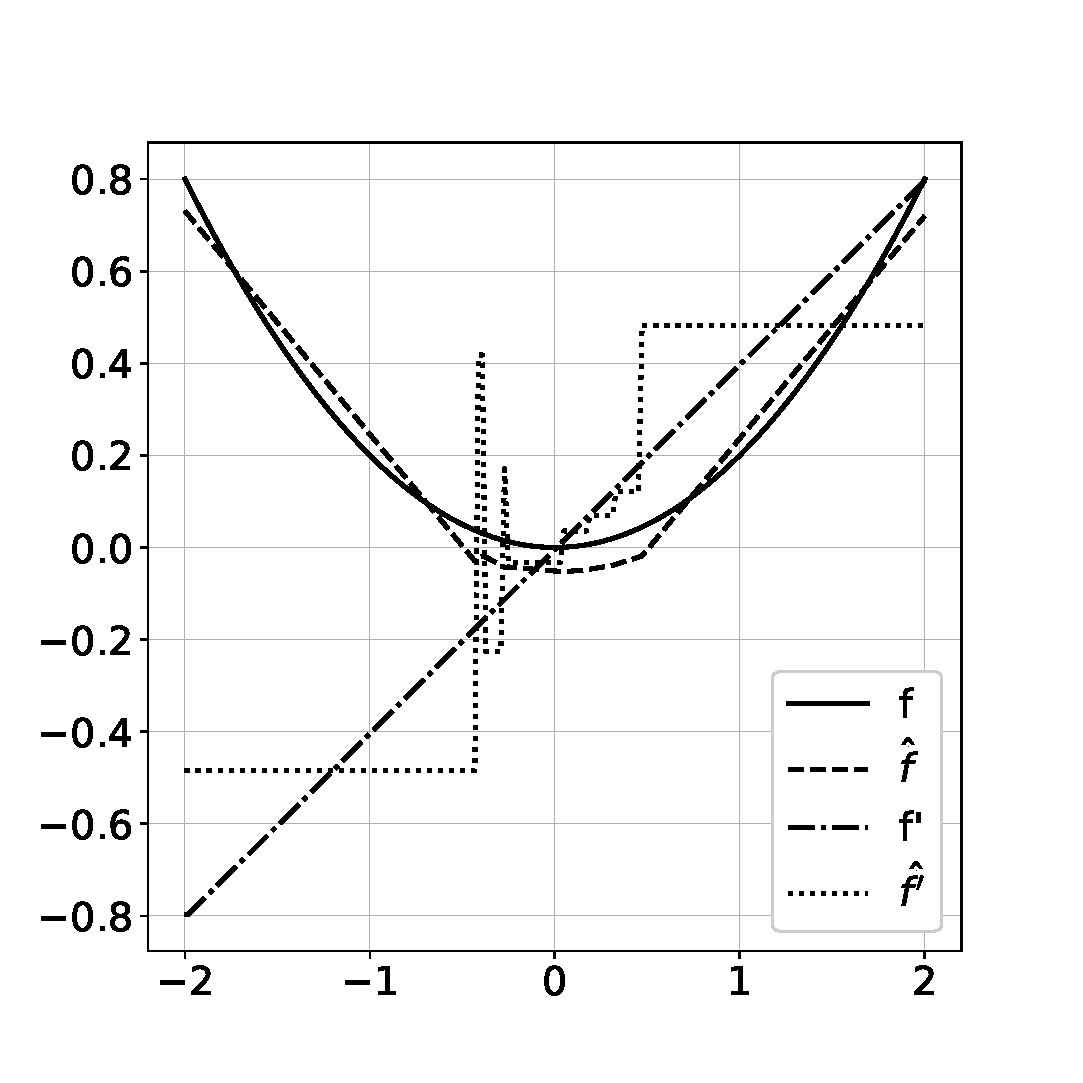
\includegraphics[trim={0.5cm 0cm 1cm 2cm},clip, width=0.328\linewidth]{pics/DerivPlot_pow_ReLEx__4eeb8531-7135-11ef-8273-4b5d8eb7968f.eps}
 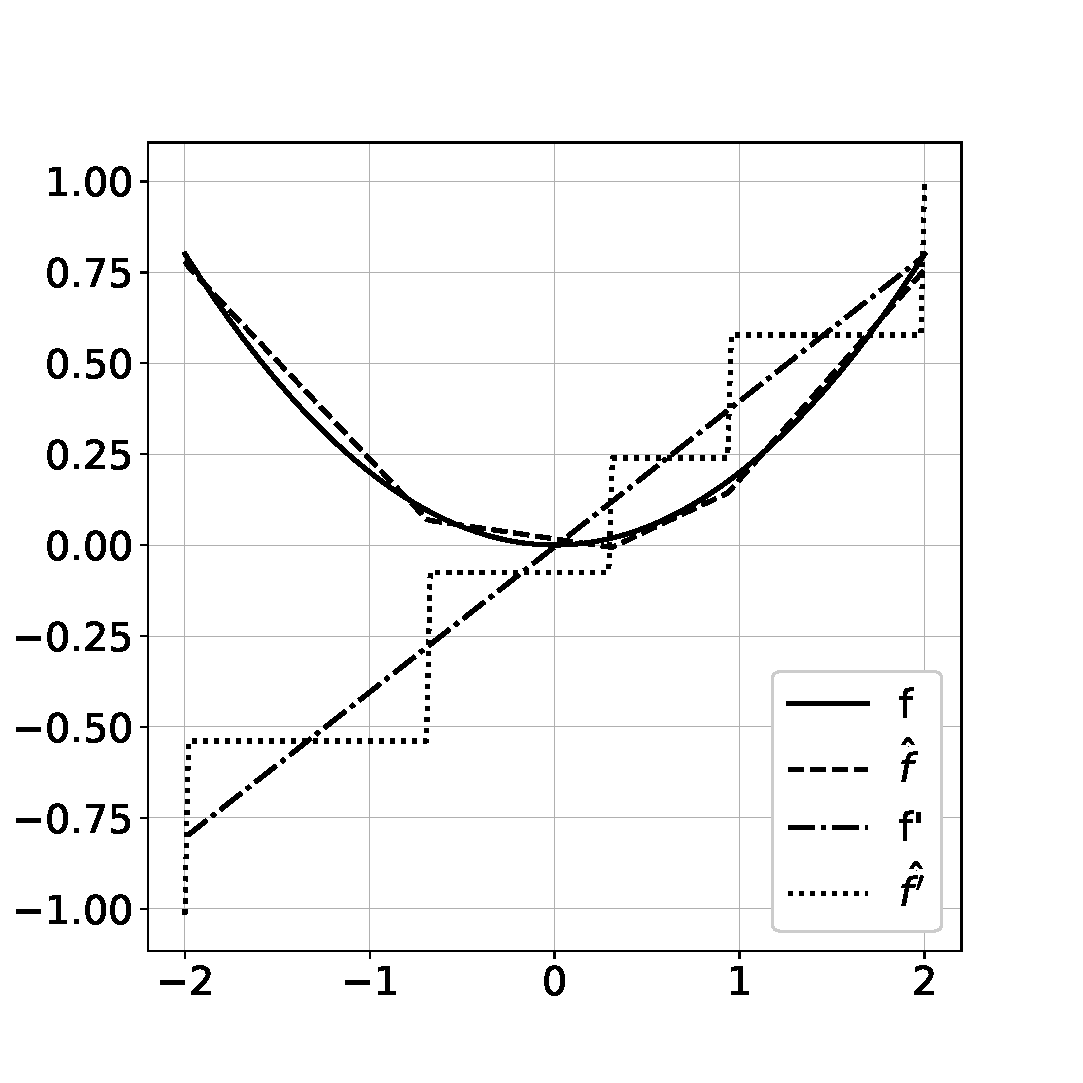
\includegraphics[trim={0.5cm 0cm 1cm 2cm},clip, width=0.328\linewidth]{pics/DerivPlot_pow_ReLEx__b0ce38b1-7135-11ef-8273-4b5d8eb7968f.eps}
 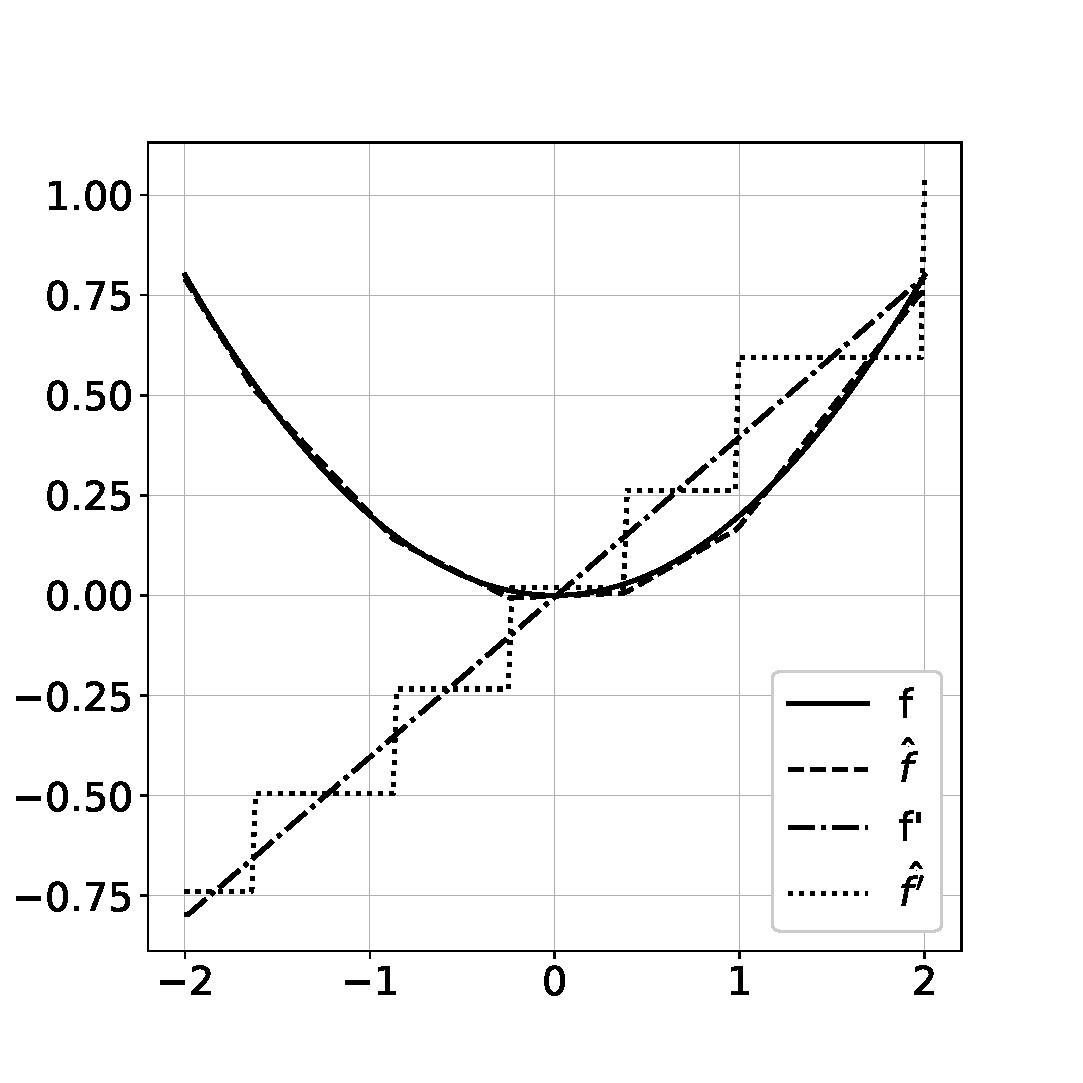
\includegraphics[trim={0.5cm 0cm 1cm 2cm},clip, width=0.328\linewidth]{pics/DerivPlot_pow_ReLEx__15c78ebb-7136-11ef-8273-4b5d8eb7968f.eps}
 
 \begin{tabular}{p{0.32\linewidth} p{0.32\linewidth} p{0.32\linewidth}}
 (a) $DATE_1$ & (b) $DATE_2$ & (c) $DATE_3$ 
 \end{tabular} 
 
 \caption{Various models trained with $DATE$ variations in (a)-(c) to approximate a quadratic function.
 %The slope of the true function derived from the data points - $f'(x)$ - and the slope of the prediction - $\hat{f}'(x)$. 
 For presentation purposes, only the output range [-1, 1] is accounted for.}
 \label{fig:runs_model}

\end{figure}


\begin{figure} 
 \centering

 \begin{tabular}{p{1\linewidth}}
 $DATE_1$
 \end{tabular} 
 {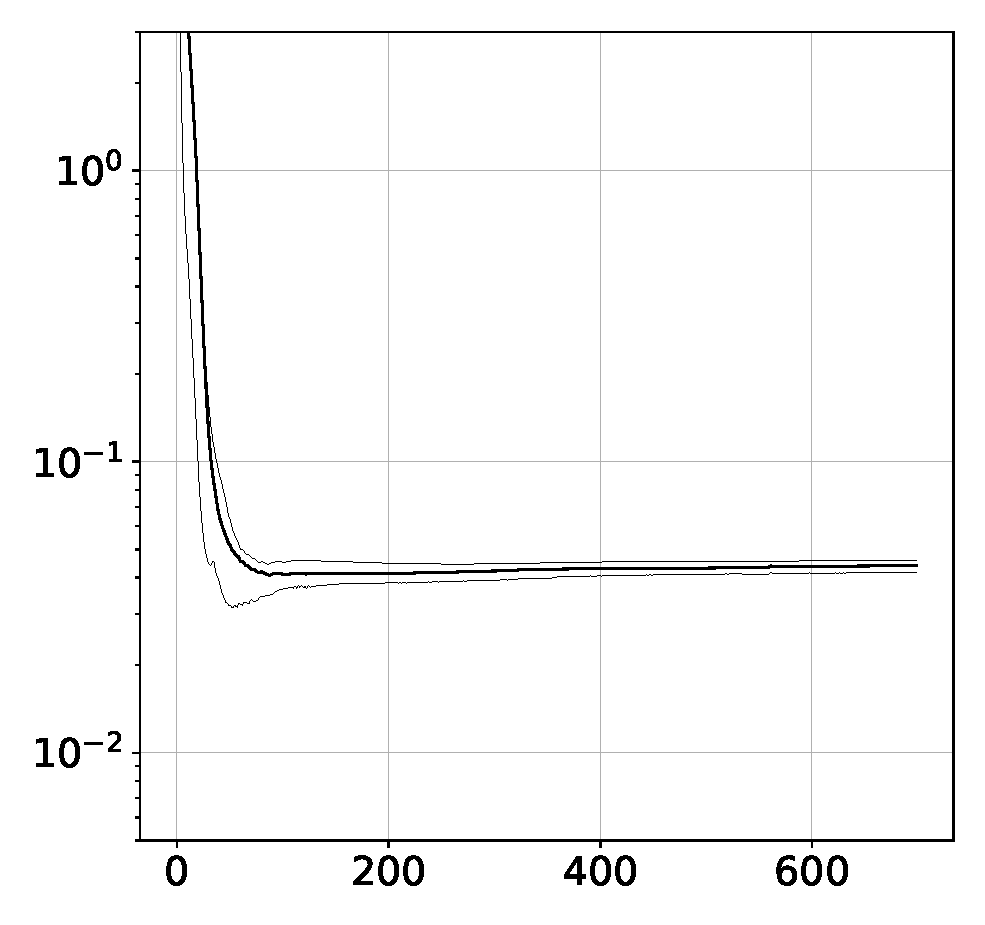
\includegraphics[trim={0cm 0cm 0cm 0cm},clip,width=0.323\linewidth]{pics/pow_dateintpow_ReLEx__4eeb8532-7135-11ef-8273-4b5d8eb7968f.eps}}
 {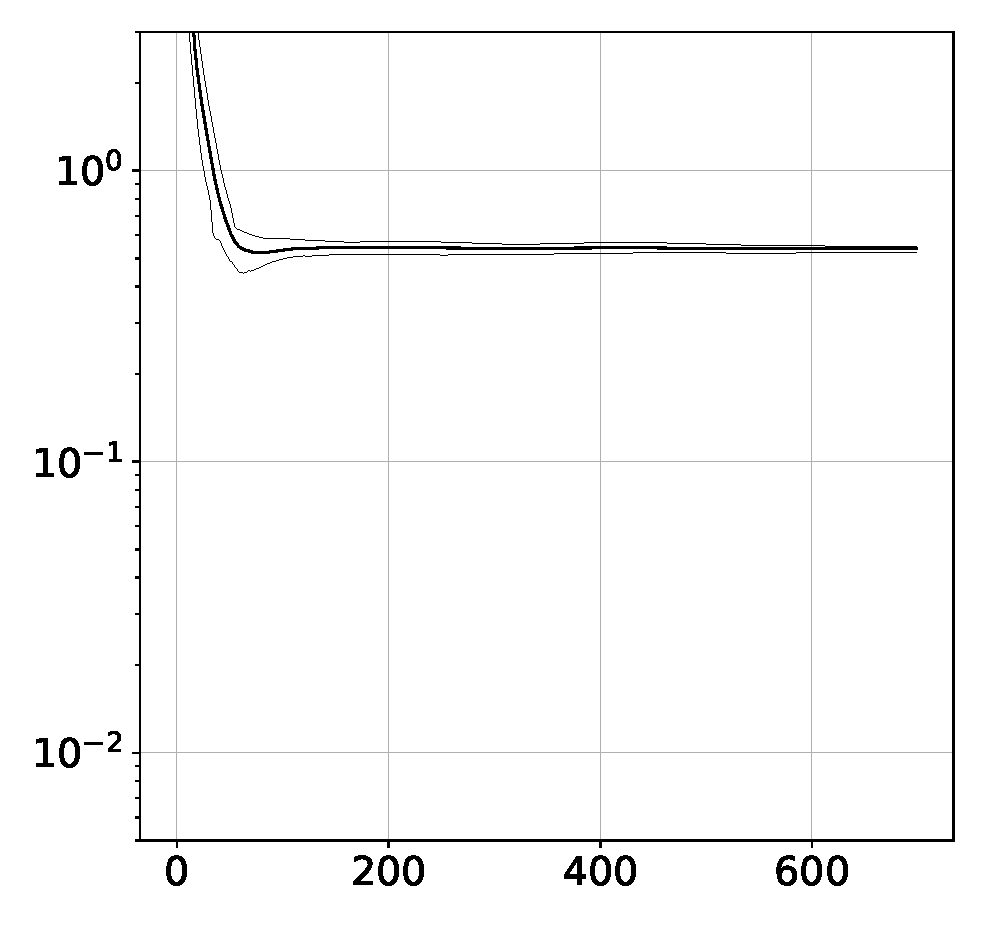
\includegraphics[trim={0cm 0cm 0cm 0cm},clip,width=0.323\linewidth]{pics/pow_dated1pow_ReLEx__4eeb8533-7135-11ef-8273-4b5d8eb7968f.eps}}
 {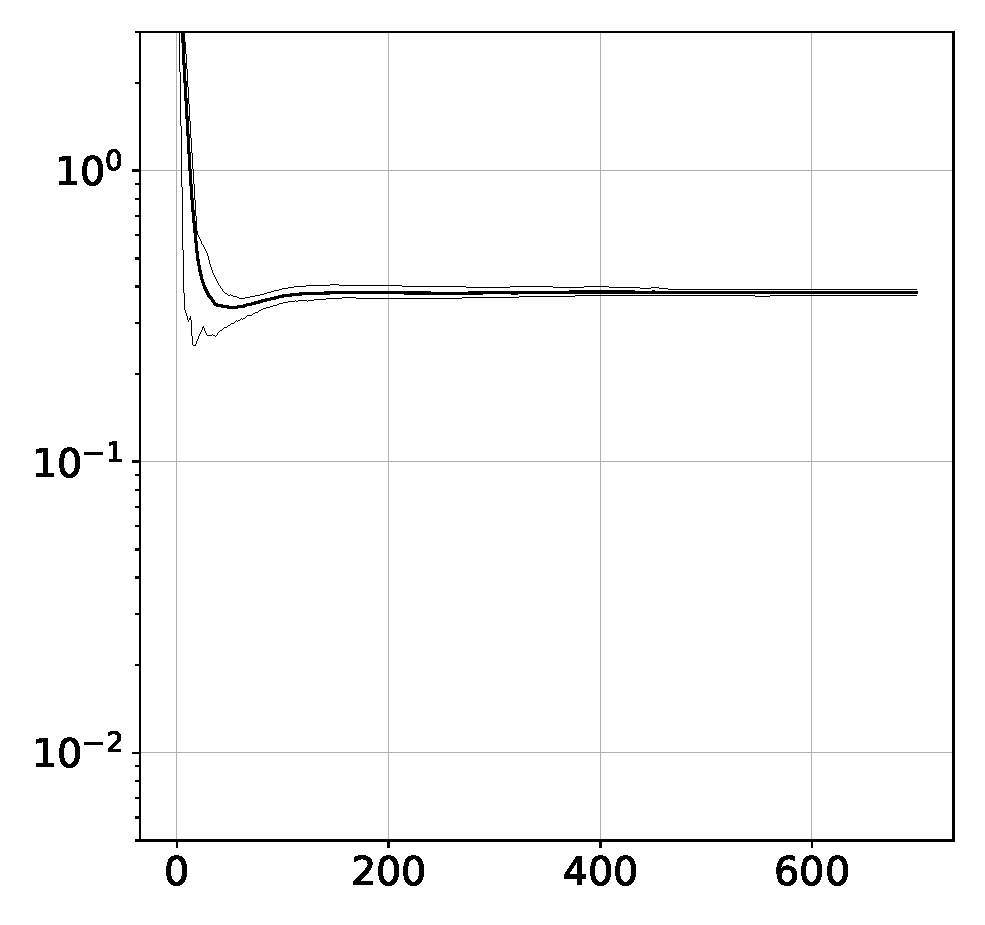
\includegraphics[trim={0cm 0cm 0cm 0cm},clip,width=0.323\linewidth]{pics/pow_datetangpow_ReLEx__4ffe1b5e-7135-11ef-8273-4b5d8eb7968f.eps}}
 
 \begin{tabular}{p{1\linewidth}}
 $DATE_2$
 \end{tabular} 
 {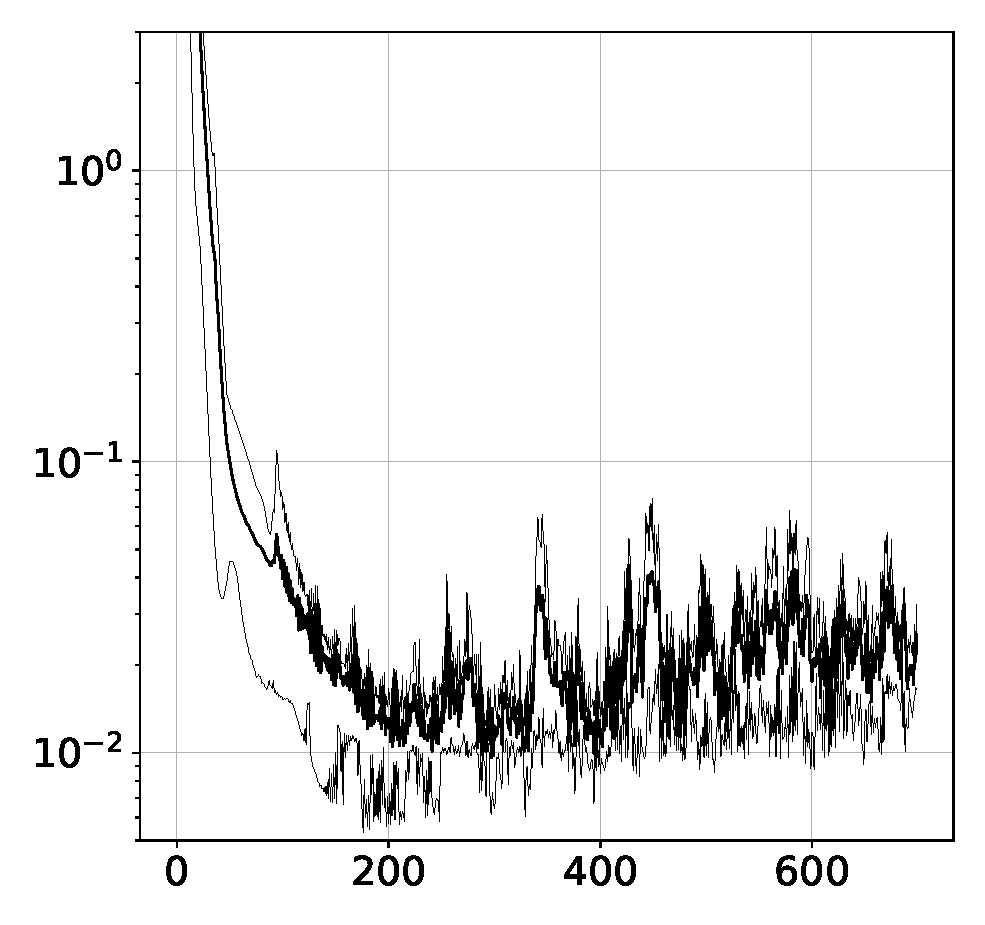
\includegraphics[trim={0cm 0cm 0cm 0cm},clip,width=0.323\linewidth]{pics/pow_date2intpow_ReLEx__b0ce38b2-7135-11ef-8273-4b5d8eb7968f.eps}}
 {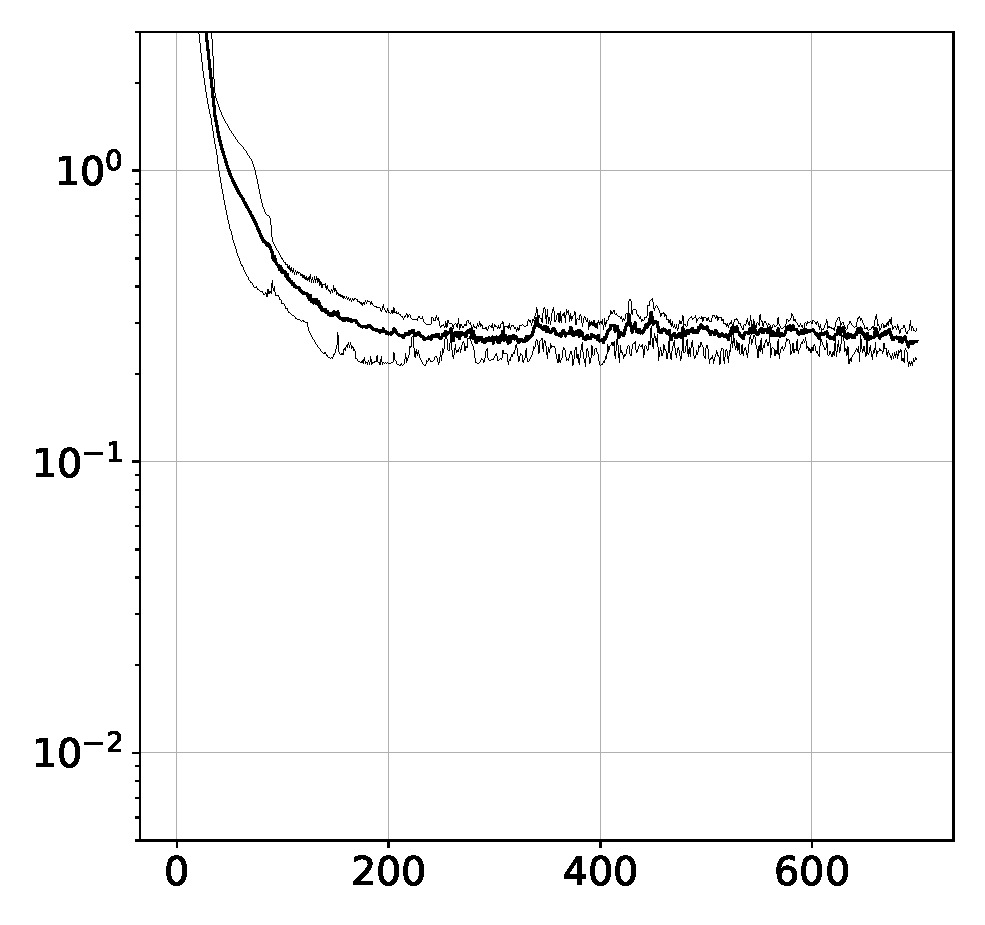
\includegraphics[trim={0cm 0cm 0cm 0cm},clip,width=0.323\linewidth]{pics/pow_date2d1pow_ReLEx__b0ce38b3-7135-11ef-8273-4b5d8eb7968f.eps}}
 {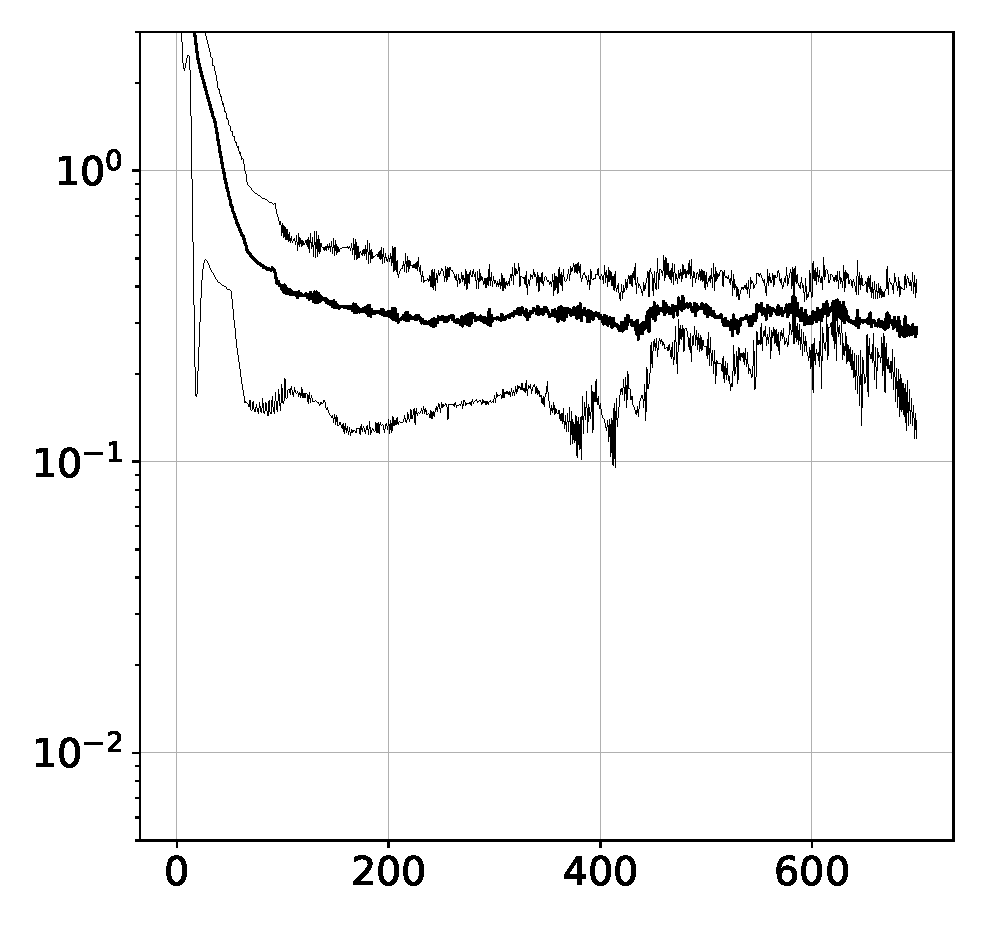
\includegraphics[trim={0cm 0cm 0cm 0cm},clip,width=0.323\linewidth]{pics/pow_date2tangpow_ReLEx__b1e55c9c-7135-11ef-8273-4b5d8eb7968f.eps}}

 \begin{tabular}{p{1\linewidth}}
 $DATE_3$
 \end{tabular} 
 {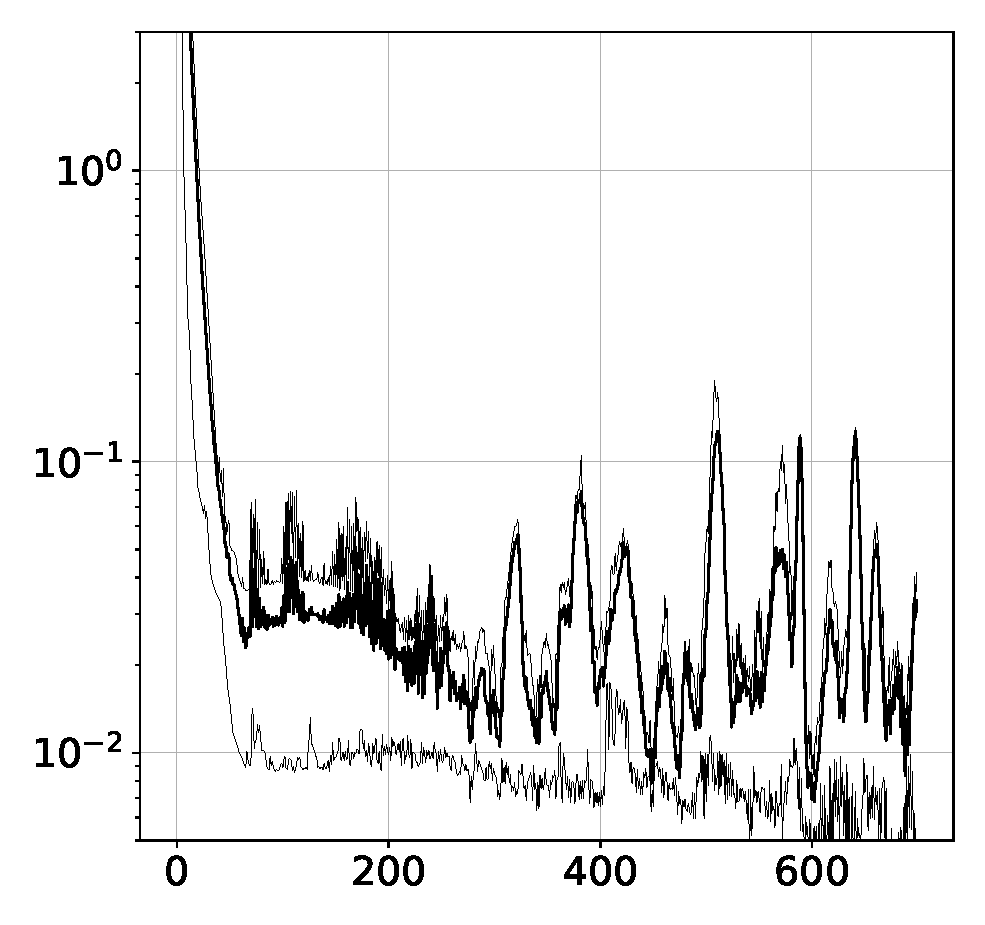
\includegraphics[trim={0cm 0cm 0cm 0cm},clip,width=0.323\linewidth]{pics/pow_date3intpow_ReLEx__15c78ebc-7136-11ef-8273-4b5d8eb7968f.eps}}
 {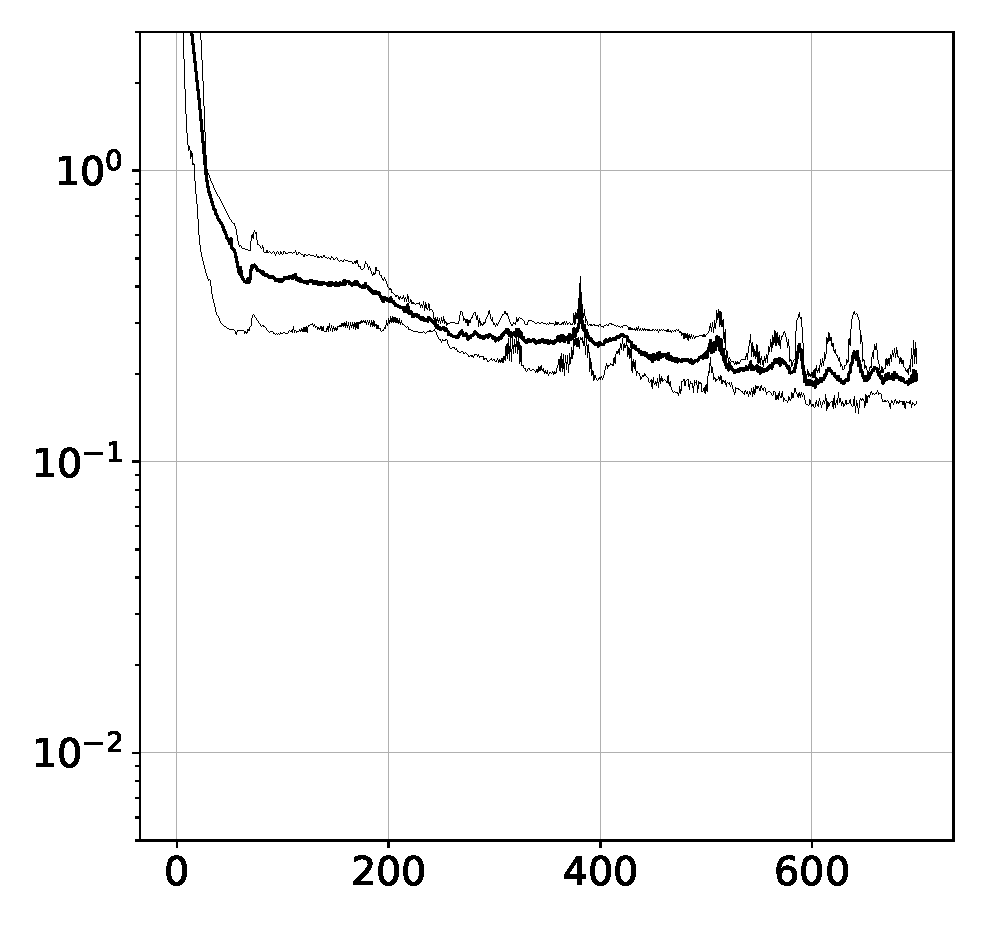
\includegraphics[trim={0cm 0cm 0cm 0cm},clip,width=0.323\linewidth]{pics/pow_date3d1pow_ReLEx__168c9818-7136-11ef-8273-4b5d8eb7968f.eps}}
 {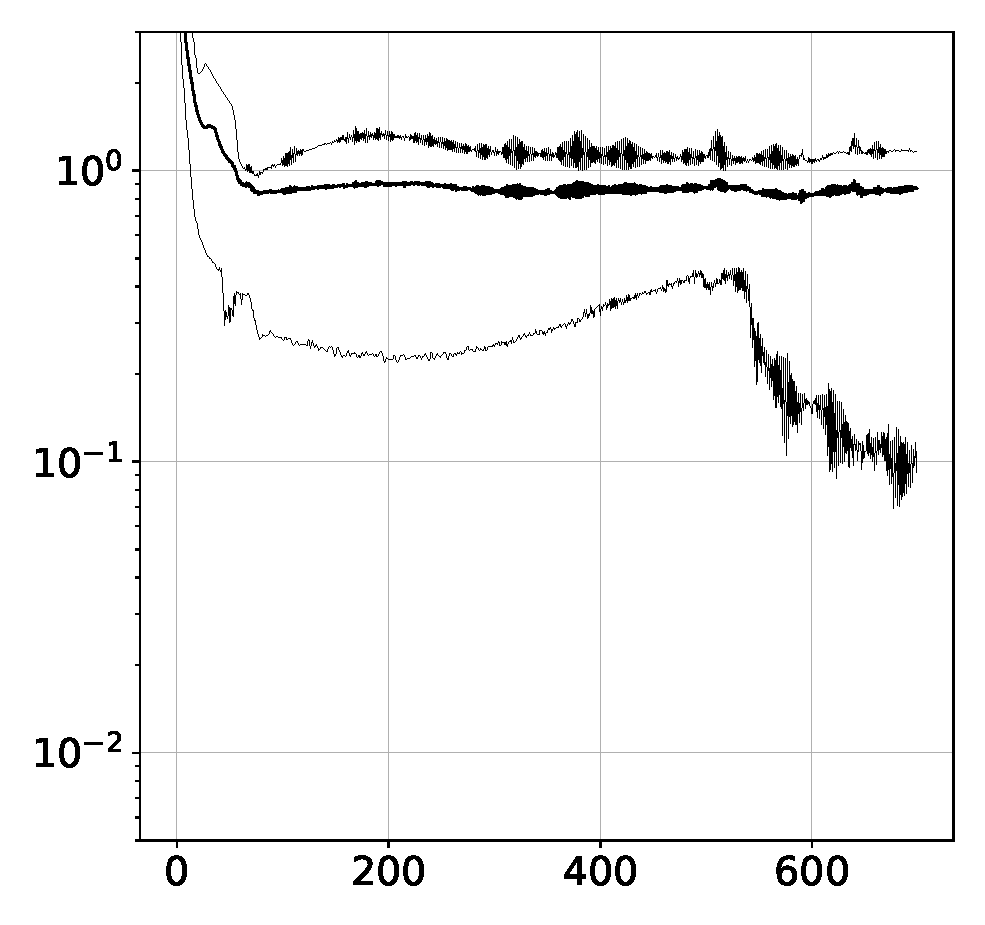
\includegraphics[trim={0cm 0cm 0cm 0cm},clip,width=0.323\linewidth]{pics/pow_date3tangpow_ReLEx__168c9819-7136-11ef-8273-4b5d8eb7968f.eps}}

 \begin{tabular}{p{0.32\linewidth} p{0.32\linewidth} p{0.32\linewidth}}
 (a) $MSE_{int}$ & (b) $MSE_{D1}$ & (c) $Tan_{ex}$ 
 \end{tabular} 
 
 \caption{Learning curves from training on scaled quadratic function for $DATE_1$, $DATE_2$ and $DATE_3$ respectively. 
 The learning represented is the average over 5 runs with 700 epochs, batch size 20. 
 The solid black line represents the average and the dotted lines represents the percentile interval [20, 80]. }
 \label{fig:results_learning} 

\end{figure}

%%%%%%%%%%%%%%

\section{Discussion}

With the $DATE$ approach, $MSE_{int}$ is in most cases improved.
In $DATE_2$ and $DATE_3$, $\Lagr_{IR}$ is responsible for pulling \emph{0-points} toward the margins of the training data range. 
We observe that using $\Lagr_{IR}$ is at least as effective as using $\Lagr_{CP}$+$\Lagr_{MR}$.
In $DATE_2$, the $\Lagr_{WO}$ is apparently still useful because its results show less variable extrapolation than $DATE_3$.

Depending on the portion of the data range close to the margins that we consider local, we can arbitrarily decide how much locally determined the extrapolation target is.
The $Tan_{ex}$ and $WLR_{ex}$ metrics for $DATE_{1,2,3}$ are lower than MSE and $ReLEx$ training for all functions considered.
%The more data are considered, i.e., the less local to the bounds of the range, the less variable the prediction.
%On the other hand, the closer data points to the bounds are considered, the more variable the prediction.
We expect $Tan_{ex}$ to be lower for $DATE_2$ and $DATE_3$, because the slope modelled with these methods will match more closely the one at the marginal of the data range. 
This is indeed the case as shown in \autoref{tab:results_theta}.

\autoref{fig:runs_model} shows the convergence of the predicted function to the true function in the range [-2, 2] on $5$ runs $DATE_1$, $DATE_2$ and $DATE_3$. These are obtained with each of the models trained over 700 epochs with batch size of 20 and Adam optimiser. 
In \autoref{fig:runs_model} we note that the slope of the model prediction in the training data range for $DATE_1$ (subfigure a) is not matching the slope of the target function as well as to $DATE_2$ and $DATE_3$ (subfigures b and c).

Lastly, \autoref{fig:results_learning} shows the learning curves for $DATE_1$, $DATE_2$ and $DATE_3$.
Compared to $DATE_1$, $MSE_{D1}$ seems to reduce faster and be less variable across multiple runs for $DATE_2$ and $DATE_3$.
With $DATE_1$ we have a more stable metrics toward the ends of the training, but at higher loss levels.
With $DATE_2$ and $DATE_3$, we observe more fluctuations toward the end of training for $MSE_{int}$, but at lower error levels.
We also observe that the $Tan_{ex}$ error is more controlled at earlier stages for $DATE_1$ but reaches lower error with $DATE_2$ and $DATE_3$.

\textbf{Limitations.}
One of the fundamental assumption in $DATE$ method is the continuation of the local linear trend at the boundary regions. 
The linear extrapolation is a popular choice in many applications because of its simplicity. 
%If the interpolation was not linear, this assumption would fall.
The choice of loss function would need to be reconsidered under a non-linear assumption.
This would involve using non-linear activation functions and higher order derivatives. 
The $DATE$ method is so far only defined for univariate situation and only for a single hidden layer. 
These are obviously severe limitation in practice and will need to be addressed. 
However, as the goal extrapolation is already not uniquely defined in the univariate case, in the multi-dimensional feature space, both, appropriate loss functions and metrics will be even more complex. 
The $DATE$ method assumes that the slope at the margins of the data range is most important for the extrapolation. 
The reliance on slope at the margins will need more attention in the case of real data, as is may amplify noise. 

%%%%%%%%%%%%%%%%%%%%%%%%%%%%%%%%%%%%%%%%%%%%%%%%%%%%%%%%%%%%%%%%%%%%%%%%%%%%%%%%

\section{Conclusions}

We propose $DATE$, a method which introduces two new loss terms to regularise the behaviour of a ReLU network, such that it produces desirable linear extrapolations beyond the margins of the training data range.
We have implemented $DATE$ in PyTorch and we have applied it to a network with a single hidden layer of $10$ neurons, single input, and single output. 
We have proposed different metrics to measure the extrapolation, as well as interpolation, performance.

In $ReLEx$ we observed that better extrapolation results were coming at the cost of higher interpolation instability.
We observe now with $DATE$ how, in general, consistent linear extrapolations paired with low interpolation error is achieved.
$DATE$ has shown some preliminary benefits in the NN case and we expect that $DATE$ can be extended to other regression methods.

Although with $DATE$ we have improved the complexity of the regularisation, we have still some limitations to overcome with future work.
Future work will include the formulation of higher order derivative, extrapolation applied to multiple dimensions, different network structures and/or other regression methods as well as working with classification problems.


%%%%%%%%%%%%%%%%%%%%%%%%%%%%%%%%%%%%%%%%%%%%%%


% ---- Bibliography ----
\bibliographystyle{splncs04}
\bibliography{references}



\end{document}